\chapter{Experimental approach}

Given the already exposed, we concentrated in Corbino ring devices, but the question remained as which heating method was to be used. The approach by Kobayakawa, \etal \cite{kobayakawa2013diffusion} is very cleaver but implies the use of high frequencies, which increases the complexity of the measuring system. Also, one could argue about how the system could follow such high frequencies, they use microwaves and a co-planar arrangement to this end. Also the themovoltage developed in the system (we will return to this concept afterwards) is measured by a central inner ohmic contact and two outer quasi-Corbino contacts, if the system has a preferred direction, are they actually measuring the proper voltage? For example in the work by van Zalinge, et. al. \cite{Zalinge2003} it is argued that the thermopower is not isotropic, again, more on this to come.

It was decided to opt for a very conservative heating system, a heating resistor to be included outside the mesa. And two approaches were considered, 1- a central heater or 2- a outer heater. The advantage on the second was that could be designed to have a much greater power, but would be hard to ensure its homogeneity, the termination would include a possible anisotropy (has to be open at the end), between some other electrical possible effects as capacitance \textcolor{tmagenta}{incluir referencia a la figura del heater por fuera (buscar el diseño que había hecho)}, inductance and such. 
So, a central heater was decided, which had to be small to resemble as much as possible a point heating system and support as much power as possible to overcome the cooling power of the cryostats to be used. For example, in the case of a wet \(^3\)He cryostat, in one hand the Helium would fight very hard against heating, but it is also possible that increasing the heating power ends in the Kapitza effect \textcolor{red}{citar acá dicho effecto} that could suddenly increase dramatically the heating power, taking the system out of regime or burning it. There, the He becomes gas, icreasing the heat capacity, increasing its temperature and resulting in an increased temperature transfer to the sample, because of both, the gas and the crystal.

\subsection{Experimental set-ups}
\label{subsec:experimental_setup}
Several measurement set-ups were tested. Usually in the laboratory we perform a regular DC measurement when working on Hall-bar samples. But in the case of thermopower it became nearly mandatory to switch to an AC approach, Fig.~\ref{fig:corbino_exp_setup}. Since we committed to a central heater and we must measure voltage and temperature responses one finds a two-fold problem: how to only measure the thermopower (thermovoltage) response \textit{only} and how to measure acurately the resulting temperature gradient produced by the heater.

\begin{figure}
    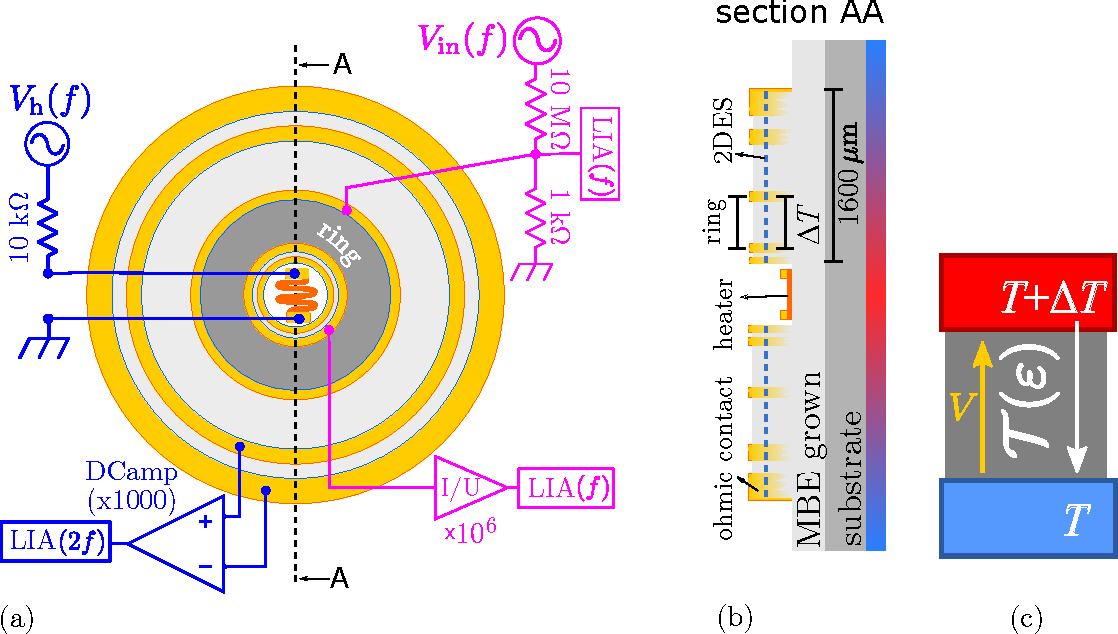
\includegraphics[width=1\textwidth]{figures/experimental/cobino_exp_arangement.pdf}
    \caption{A typical device scheme is shown. Notice the several concentric Corbino devices, they act independentrly during measurements (see text). (a) Experimental setups: \textcolor{blue}{blue} configurations are intended to measure thermopower, \textcolor{magenta}{pink} configuration is used to produce conductance measurments of the system. We will denote the innermost Corbino ring 1, then 2, and the outermost will be ring 4. (b) Section cut AA of the schematic device depicted in (a), notice that the central resistive heater is outside the mesa and will induce a radial heating on the samples. (c) Scheme of the two contact device we think of when modeling the system. Being the hot contact the inner ohmic Corbino contact, and the cold one the outer ohmic Corbino contact. \textcolor{red}{incluir luego un panel adicional con fotos de los dispositivos.}}
    \label{fig:corbino_exp_setup}
\end{figure}

The first problem has been overcome before by Molenkamp \etal \cite{molenkamp1993QPCthermal}, when studding thermoelectric responses in QPCs. They demonstrated that one can measure the thermovoltage responses by lock measuring the second harmonic response of the system to the heating device. 

So, an AC voltage $V_\text{h}$ resulting in a current $I(t)$ of frequency $f$ is applied to the heater, and it's seccond harmonic response will be measured by a lock-in amplifier (LIA)
\begin{equation}
    \label{eq:heater_current}
    I(t)=I_0\sin(\Omega t + \varphi), 
\end{equation}
with \( \Omega= 2\pi f \), and \( \varphi \) a possible arbitrary phase. This translates into the power,
\begin{equation}
    \label{eqs2}
    P(t)= \frac{R I_0^2}{2} \left[1- \cos(2 \Omega t + 2 \varphi) \right],
\end{equation}
where \(R \) is the heater resistance.

Thus, a temperature bias is generated between the heater and the external rim of the structure which has a constant component and one that oscillates with the frequency $2 f$. 
In \textcolor{red}{citar seccion dependencia potencia con temp medida}, we show that there exists a linear relation between the power and the temperature bias. Therefore, it is natural to assume the following behavior for the temperature bias,
\begin{equation}
    \label{eq:deltaT_time}
    \Delta T (t) = (\Delta T)_0 - (\Delta T)_2 \cos (2 \Omega t + 2 \varphi).
\end{equation}

At very low frequencies and under ideal conditions, $(\Delta T)_2$ should be independent of the frequency and equal to $(\Delta T)_0$. We shall come back to this point later on. 
Consequently, the developed thermovoltage has a constant component plus an oscillating component of frequency $2f$, this is 
\begin{equation}
    \label{eq:vtp_time}
    V_{tp}(t)=V_{ tp \, 0} - V_{tp \, 2} \cos (2 \Omega t + 2 \varphi).
\end{equation}

The experimental setup is designed to measure the oscillating component $ V_{tp \, 2}$ of the thermovoltage. 
The Seebeck coefficient $ S={\cal L}_{12}/{\cal L}_{11} $ relating the thermovoltage with $ \Delta T $ depends on the microscopic mechanisms behind the transport processes. 
Within linear response this quantity is expected to be the same for the constant and oscillating components of $ \Delta T $ and $V_{tp}$. 
Notice that in this type of measurement there is a $3\pi/2+\varphi$ phase lag between the oscillations of the injected current and the measured thermovoltage. 
The measurements we show in this text have a $\varphi=0$ injected signal phase and the corresponding 2nd harmonic in the signal of $ V_{tp} $ has a phase lag of $3\pi/2$ within the Landau levels, in full agreement with Eqs. (\ref{eq:heater_current}) and (\ref{eq:vtp_time}). 

However, as we will discuss in \textcolor{red}{citar seccion vtp meas} within the gaps between Landau levels the response shows spike like voltages, which have also other phase lags, and out of phase huge responses. The origin of the latter features were a striking feature and required an important amount of work to understand. We will get back to them, but let us state that for the time being we have a culitative explanation to them, and deserves future investigations.

From the technical point of view, it is important to chose the proper frequency range. We studied the thermopower response at different frequencies and found an upper limit at $f = \SI{100}{\hertz}$, i.e. $2f = \SI{200}{\hertz}$ where the voltage started to decrease with increasing frequency. On the other hand, the total cryosystem has a characteristic thermal-relaxation corresponding to a frequency below \SI{1.5}{\hertz}. These two frequencies determine the frequency range that could be used during thermopower measurements, we have use \SI{13.838}{\hertz} unless otherwise stated.

The conductance measurements were not constrained by these limits, because the additional power dissipation was always negligible. A higher frequency of \SI{113}{\hertz} increased the accuracy and reduced the measurement times, which was particularly relevant for the temperature calibration, to be discussed in section~\ref{temperature_corbino}. In the QHE regime the internal resistance of the thermal voltage can become very high. Its measurement requires a DC amplifier with very high input impedance. We use an amplifier with about \SI{10}{\tera\ohm} input impedance and differential guarded inputs \cite{Maerki2017}.

We verified that the measurement of the voltage across the radius of the device is indeed generated by a thermoelectric effect rather than being induced  by a time-dependent magnetic field. The latter effect would actually be the experimental realization of Laughlin's {\em gedanken} experiment \cite{laughlin1981quantized}. According to this, a time-dependent magnetic flux threading  the Corbino ring would induce an electrical field given the induced emf by Faraday law, causing eddy currents circulating along the circumferences of the structure, which would lead to the development of a radial Hall voltage. Such voltage would depend on the time-derivative of the magnetic field. 
Thus, the measurements have been performed by changing the magnetic field in steps using different waiting times to allow the thermovoltages and magnet to stabilize.

In addition, we made voltage measurements in the thermovoltage configuration (see Fig.~\ref{fig:corbino_exp_setup}) both within the Landau levels and within the gapped regions with the magnetic field pointing in opposite orientations.
We did not find any signature of an effect due to a time-dependent magnetic flux, as the ones discussed by Dolgolopov, \etal\cite{dolgopolov1992quantum,dolgopolov1993charge}. There they produce measurements in both magnetic field directions, and showed that in such cases we could expect a toothsaw-like response wich sign would be dependant of the magnetic field derivative, as sown in Fig.~\ref{fig:dolgo}.

\begin{figure}
    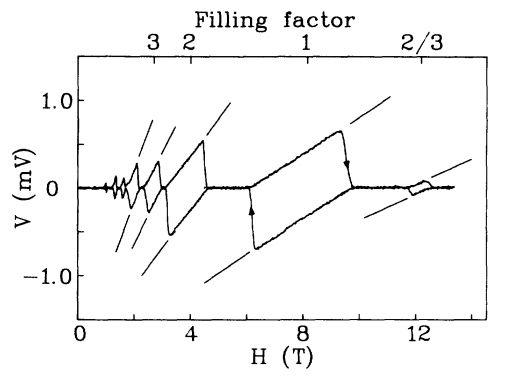
\includegraphics[width=0.7\textwidth]{figures/experimental/dolgopolov_01.png}
    \caption{Expected voltage respose in the case of time-dependent magnetic flux, it translates in an iduced electrical field (emf by Faraday) resulting in circulating eddy currets and further Hall voltages. Note that such effect is dependant of the direction of the magnetic field derivative. Figure reproduced from Dogolopov, \etal \cite{dolgopolov1992quantum}, Copyright (2022) by the American Physical Society \url{https://doi.org/10.1103/PhysRevB.46.12560}. Original caption: Potential difference between inner and outer contacts in incresing and dcreasiing magnetic field. Sample 5, \( T = \SI{25}{\milli\kelvin}\). The straight lines show slopes expected from Eqs. (1) and (2) for filling factors \( 2/3, 1, 2, 3, 4.\).  }
    \label{fig:dolgo}
\end{figure}



\subsection{Power dependance}
\label{subsec:powerDependance}

Since the thermopower is the consecuence of the temperature difference between the contacts under study, it should scale on power. 
Equation \textcolor{red}{citar equación potencia heater} states that the power at the heater will be transferred to the substrate and will produce a proportional temperature difference. In the case of the cold finger configuration one could think of radiation too, but some basic calculation of the Stefan-Boltzmann law shows that its contribution is neglegible 
\begin{equation} 
    \label{eq:stephanBotlzmann}
    \begin{split}
        P   &= \epsilon \sigma A T^4 \\
            &= (1) (\SI{5.67e{-8}}{\watt \metre^{-2} \kelvin^{-4}})(\pi(\SI{250}{\micro\meter})^2 ) (\SI{1.6}{\kelvin})^4 \\
        P   &= \SI{7.3e-5}{\nano\watt},
    \end{split}
\end{equation}
this is orders of magnitude below usual heating powers used in this work, which are avobe the \unit{\nano\watt}. In \ref{eq:stephanBotlzmann} we assume the worst case of a perfect emissivity, a larger round heater of \SI{250}{\micro\meter} radius and the worst possible base temperature.
So it is fare to assume that we transfer all heater power to the substrate, being radiation effects negligible. 

Now, such heating could or not be transferred to the 2DES. Given that our lowest temperature is around \SI{260}{\milli\kelvin}, no decouple of the electron-phonon system should be expected. Also, given the porperties of our system no pohonon focussing effects are expected \cite{anderson2012phonon,ramsbey1988phonon,karl1988imaging}. Such effects should have been observed during measurements given the variety of devices we tested, we measured Corbinos of different radius and thin, thick and Cr-doped samples, we did not find any signature of such possible efect.\textcolor{red}{inlcuir cita, también, tal vez incluir acá el detalle de las dopadas con Cr y el thinning en vez de hacerlo en el anexo únicamente.} 

Given the previous discussion, it is fare to assume that the heater power should be completely transferred to the substrate resulting in a temperature gradient in our Corbino 2DES. An then, we can expect a direct relation between temperature gradients and power applied. We show usual measured responses at different temperatures in the figures \ref{fig:D170522B_thick_power_01,fig:D170522B_thick_power_02,fig:D190130A_Cr_power,fig:F150709B_power_01,fig:F150709B_power_02}. Unless stated, all measurements will be standard, in the sense that our usual magnetic resolution measurements were \SI{10}{\milli\tesla}.

\textcolor{red}{Juntar las imágenes de potencia en tres paneles (uno por muestra) y mejorar los tamaños de letra. Hacer uno específico para la zona de los LL. Tal vez usar directamente el que pusimos en el paper y que va en modeling.}

\begin{figure}
    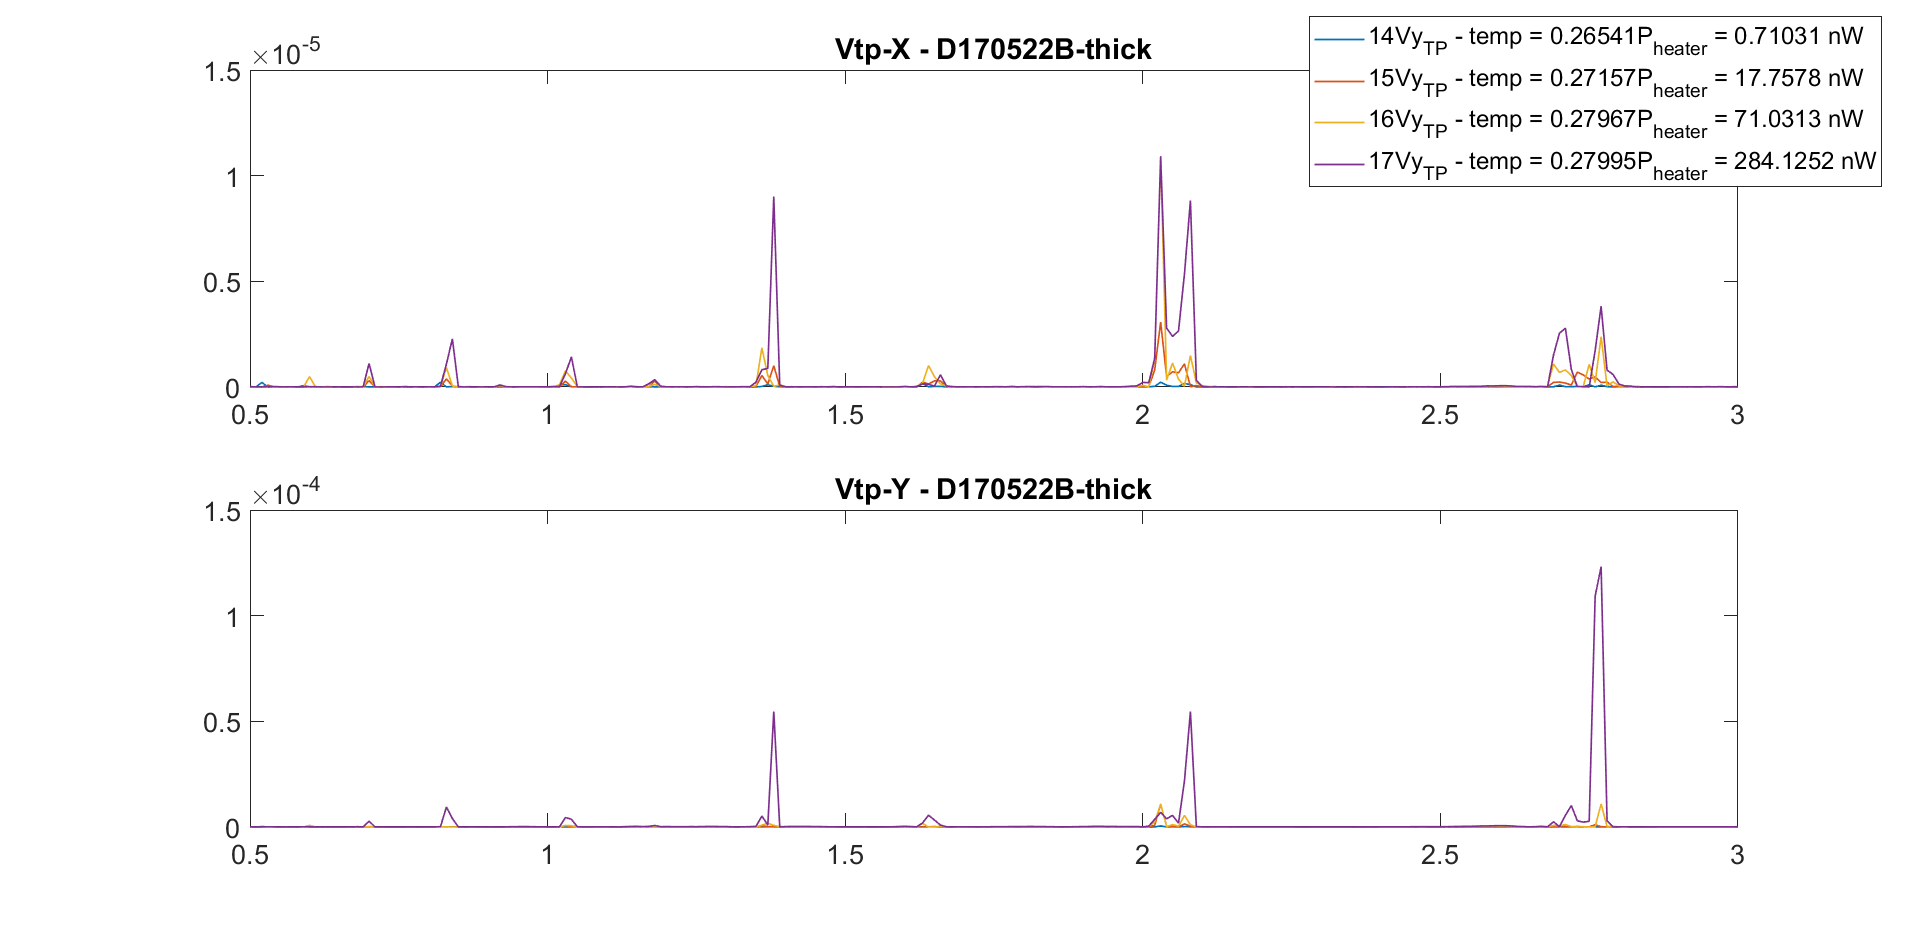
\includegraphics[width=1\textwidth]{figures/experimental/powerDependance/D170522B-thick-cambio-potencia-01.png}
    \caption{caption.}
    \label{fig:D170522B_thick_power_01}
\end{figure}


\begin{figure}
    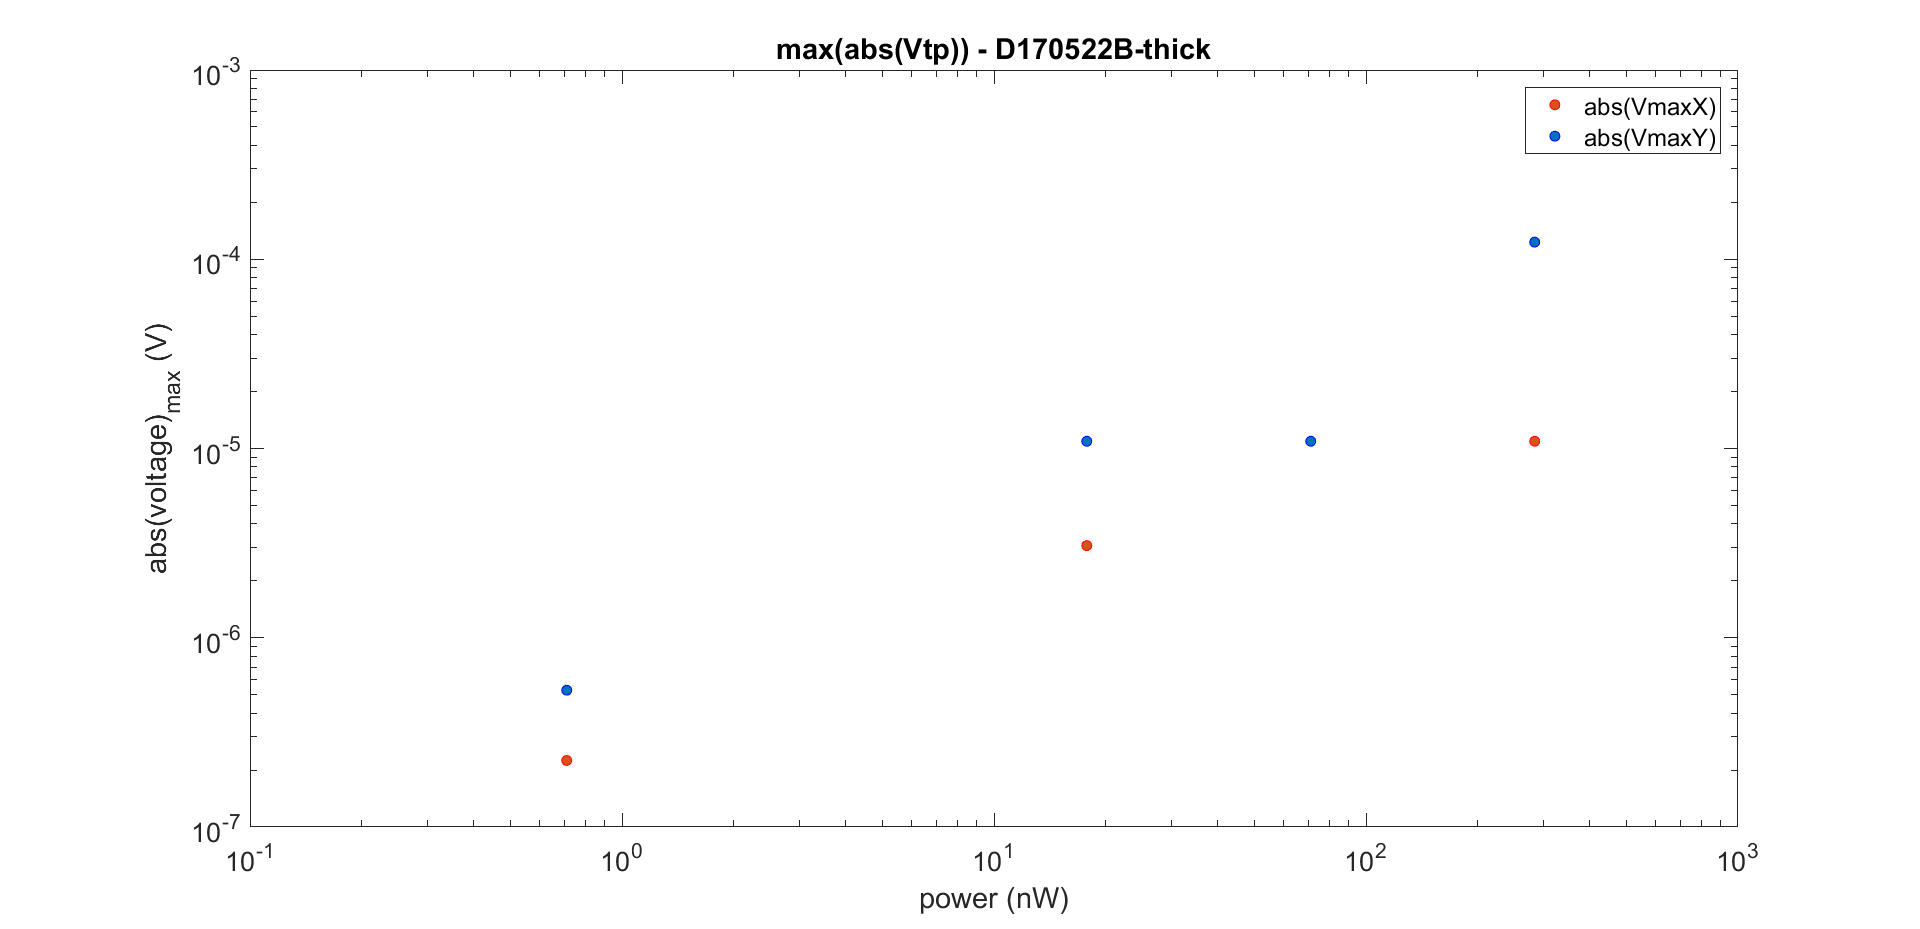
\includegraphics[width=1\textwidth]{figures/experimental/powerDependance/D170522B-thick-cambio-potencia-02.png}
    \caption{caption.}
    \label{fig:D170522B_thick_power_02}
\end{figure}


\begin{figure}
    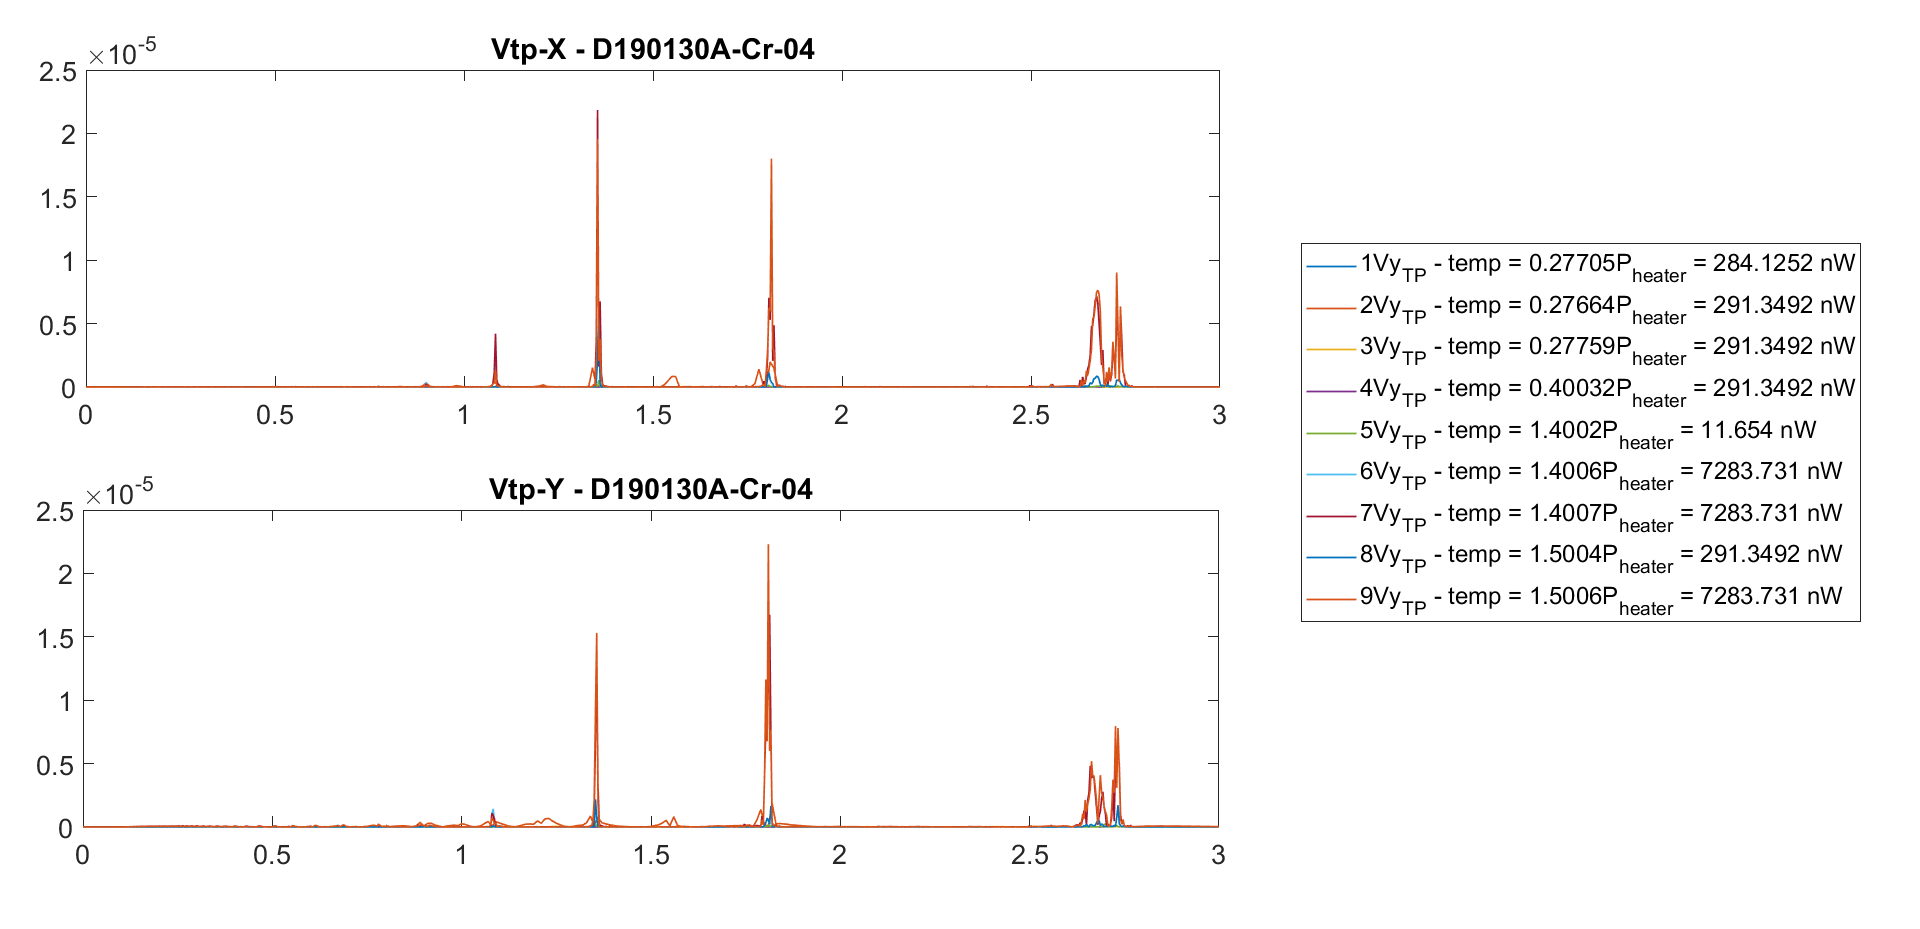
\includegraphics[width=1\textwidth]{figures/experimental/powerDependance/D190130A-Cr-04-todas.png}
    \caption{caption.}
    \label{fig:D190130A_Cr_power}
\end{figure}


\begin{figure}
    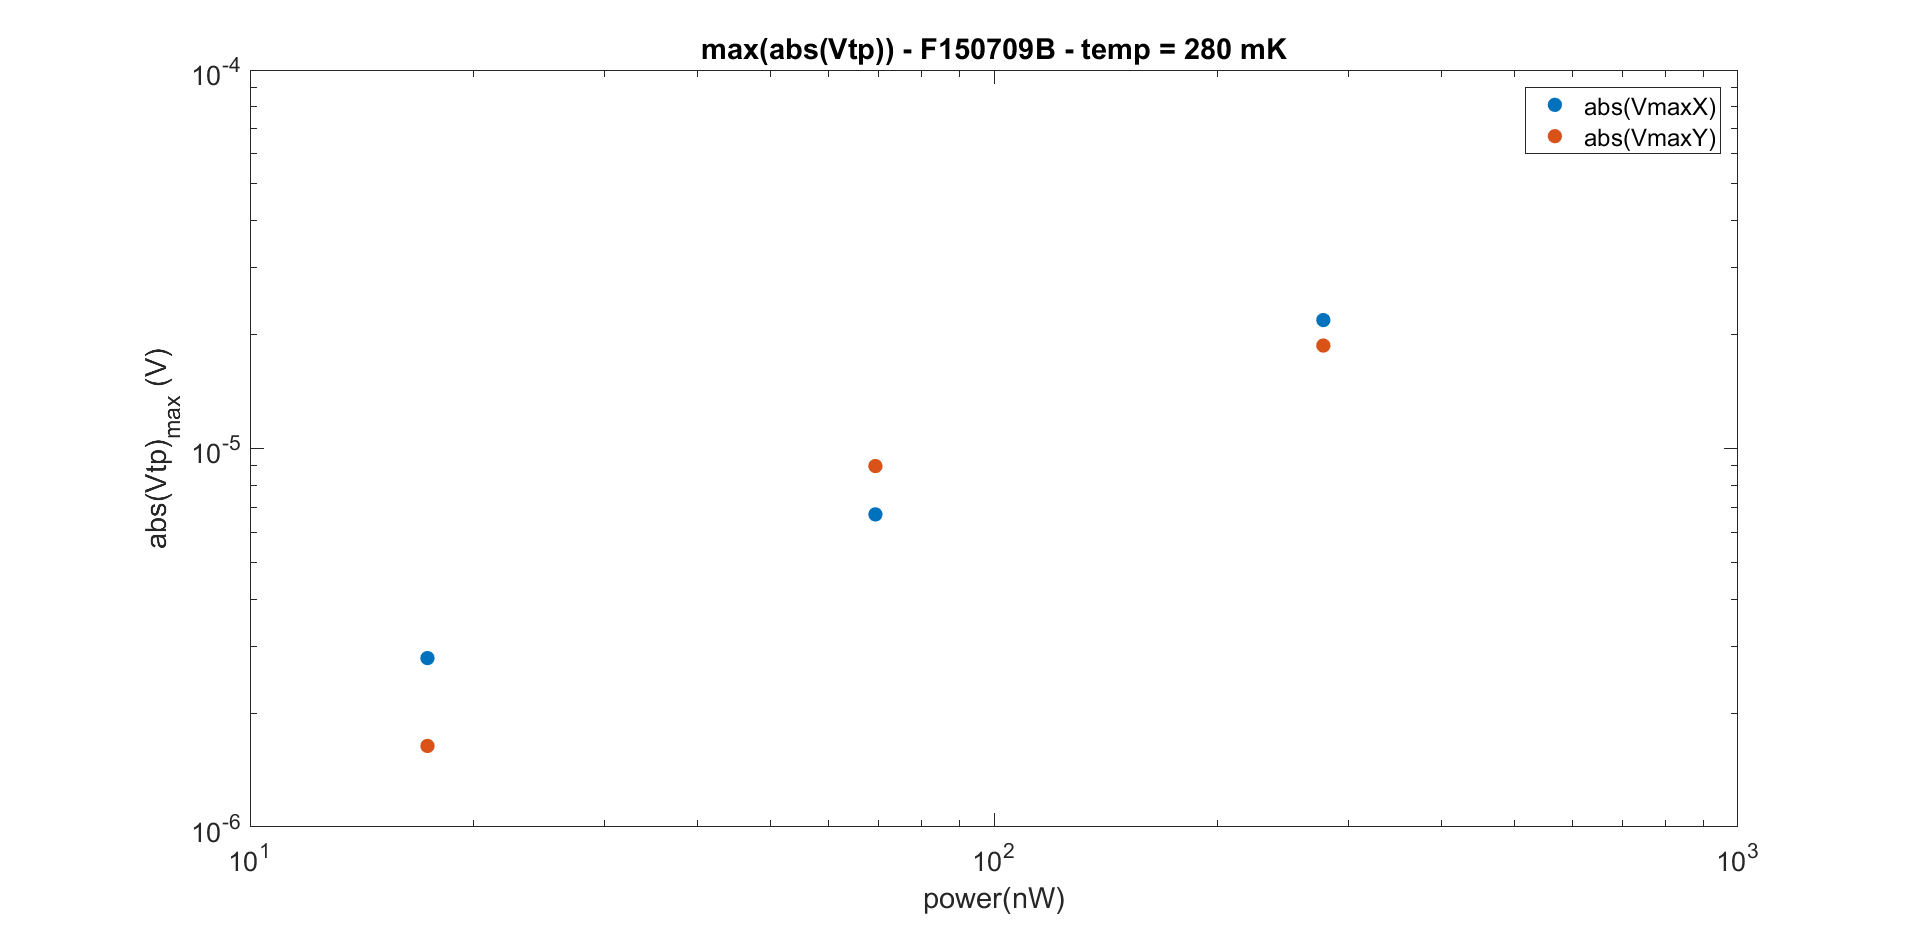
\includegraphics[width=1\textwidth]{figures/experimental/powerDependance/F150709B-cambio-potencia-01.png}
    \caption{caption.}
    \label{fig:F150709B_power_01}
\end{figure}

\begin{figure}
    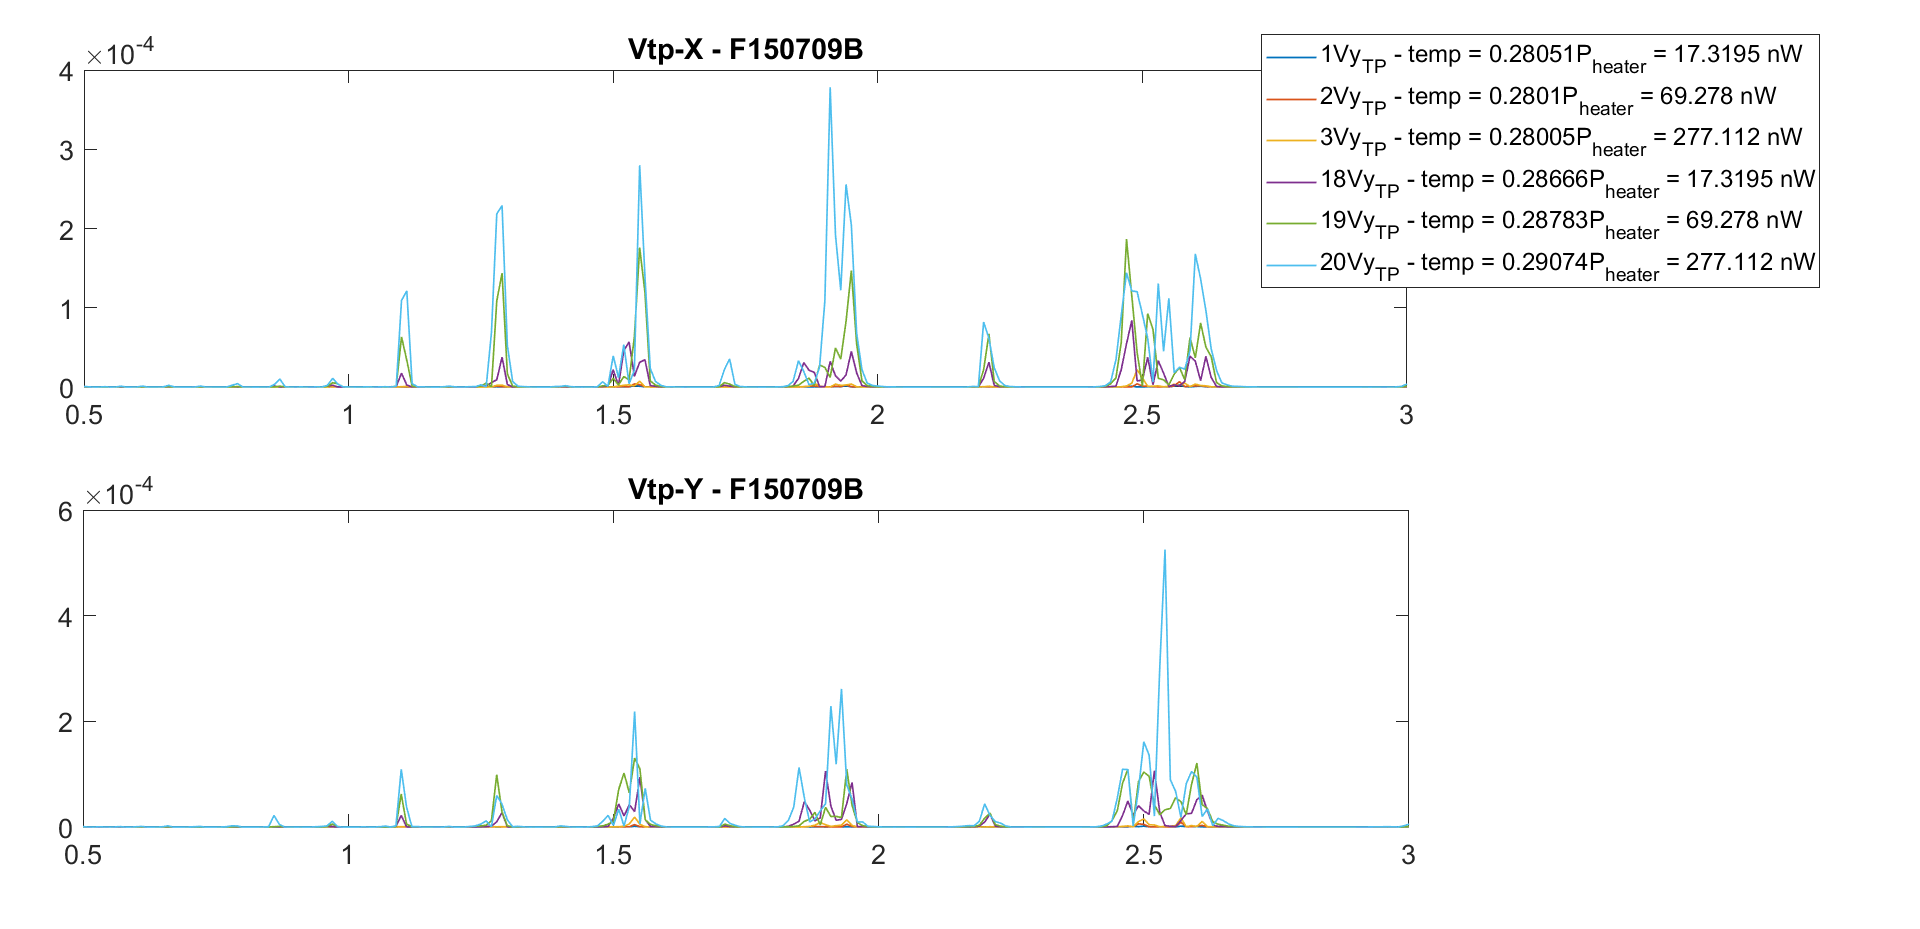
\includegraphics[width=1\textwidth]{figures/experimental/powerDependance/F150709B-cambio-potencia-02.png}
    \caption{caption.}
    \label{fig:F150709B_power_02}
\end{figure}

As shown, in all cases the response of the system depends on the power applied, as expected. What was not expected is the huge response in the gap, here shown in the \( \vtpx \) plots, that scales as the one of \( \vtpy \) in the gap. We shall come back to this in \textcolor{red}{citar la sección donde se discute esto.}. We will come back to the power dependance in \textcolor{red}{citar ch:modeling, fig: power dependance con modelo}, where whe show how the developed model predicts the different responses at different heater power.


\section{Thermovoltage and conductance measurements}

Up to now we have discussed some aspects of the measurements but not in detail, we shall do it in this section. Coming back to the experimental setup already mentioned, let us discuss two main measurement situations initially: a- conductance measurements, and b- thermopower measurements. 

\begin{figure}
    \centering
    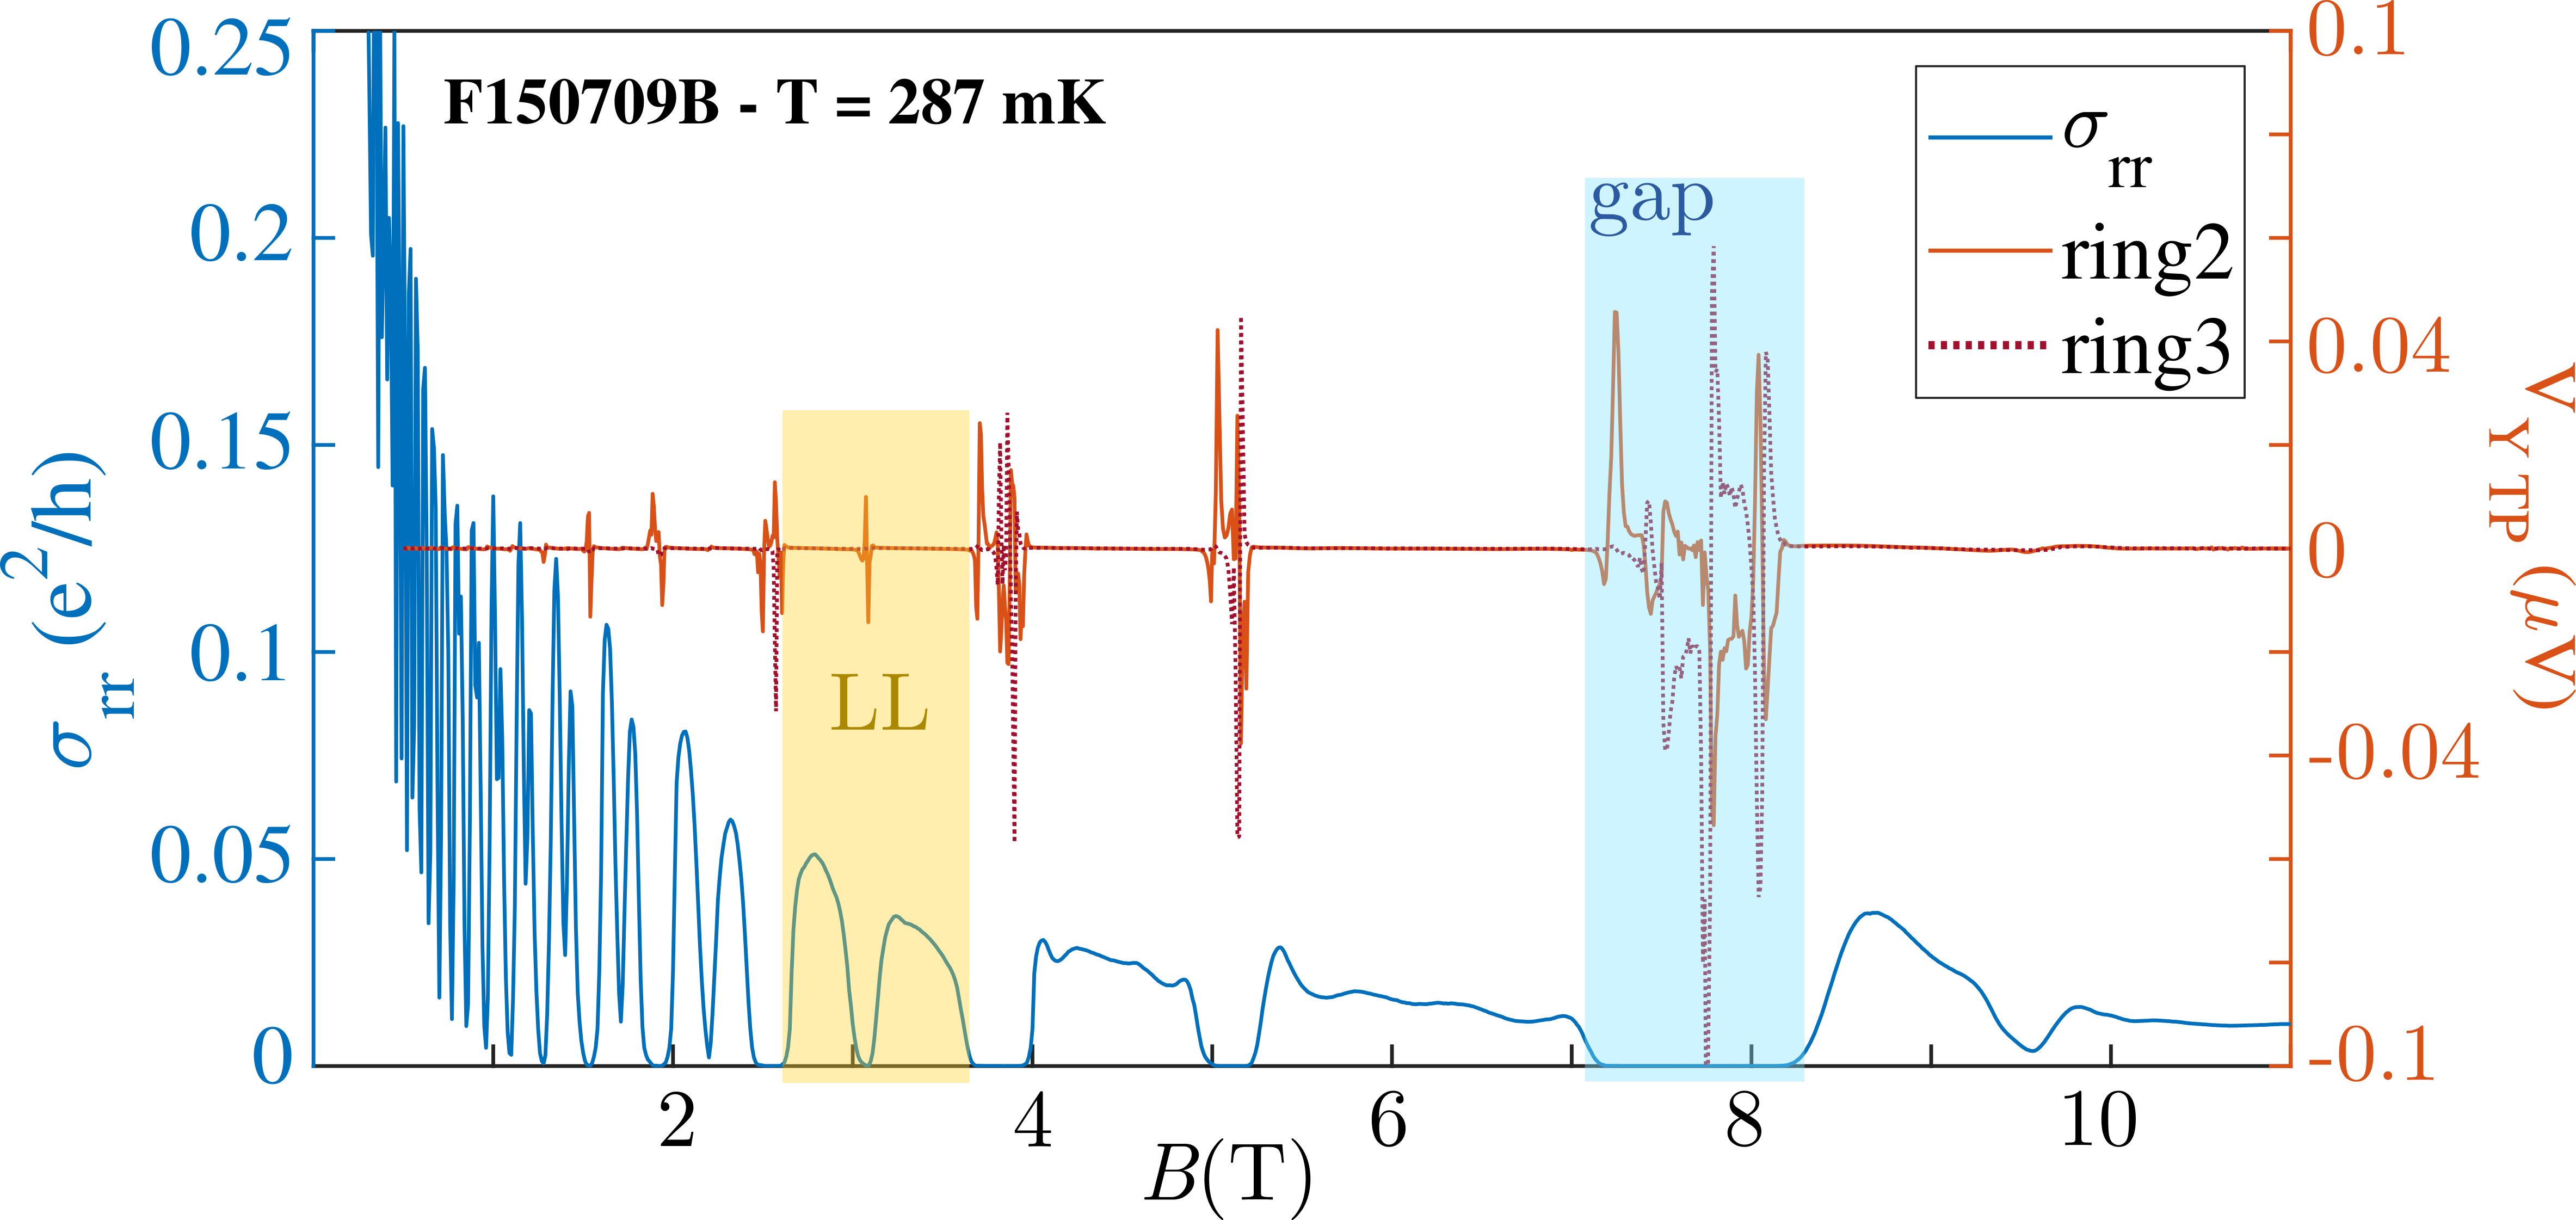
\includegraphics[width=1\textwidth]{figures/experimental/GandVtpExample.png}
    \caption{This is a typical conductance example, showing the expected behavior of the system in its different stages (LL and gap). A very schematic measurement inset is given, the actual measurement set-up is given in Fig. \ref{fig:corbino_exp_setup} \textcolor{red}{No puse los filling factor, agregar, también los N de los LL y el spin (ver el grafico del paper de corriente).}}
    \label{fig:GandVtpExample}
\end{figure}

Figure \ref{fig:GandVtpExample} shows some typical results of the conductance (blue curve) and of the \( \vtpy \), orange and reddish curves for ring 2 and 3, we introduce here this measurements to introduce to some particularities and be able to discuss later in detail the different details they have. 
In this measurements, as we increase the magnetic field the Subnikov de Haas (SdH) oscillations develop, until quantization ($G = 0$) is reached. Each bulb in this curve is the result of the different Landau levels, and as the magnetic field reaches higher values ($B \sim \SI{1}{T}$) full quantization is obtained and so the mobility gap completely displayed by the conductance (conductivity in this plot). Also, it is important to note the point at which the spin splitting of the system can be observed ($B \sim \SI{1.5}{T}$ for this sample and temperature). This is why the LL in yellow is marked over two conductance increases, they belong to the same LL but having different spin. This measurements were produced by applaying a voltage to the inner ohmic contact of ring 2 while measuring the current circulating at the outer contact 
\textcolor{red}{tal vez conviene nombrar cada contacto con un número y hacer un gráfico.}
by means of the I/U amplifier locked to the excitation voltage at a frequency $f = \SI{113}{\hertz}$. 

Most measurements in this work will focus in the region \SIrange{0.5}{3}{\tesla}, because the measurements were very time consuming, for example figure \ref{fig:GandVtpExample} required an overnight measurement for $G$ and a complete day for $\vtp$. Also, we wanted to avoid the inclusion of FQHE effects on this stage of the developments, since many more possible effects could become relevant.

Regarding the $\vtp$  measurements in Fig. \ref{fic:GandVtpExample}, it was not expected that the system presented such large and complex behavior in the gap. Another point (not shown in this figure) is that the out of phase response in the gap was of the same magnitude as the one shown, another unexpected result that we shall discuss in the next chapter. Also note that ring 2 and 3 are consecutive and the change in sign, this are floating measurements, so there can be a change (overall phase) modifying the output. 


We performed measurements at INTI and at ETH-Zürich (Prof. Wegscheider's group), the measurements set-ups at each location was different, depending on the equipment availability. In the case of INTI, we use a wet $^3$He cryostat while at ETH we performed measurements in a cold finger configuration, further instrumental details are given in \ref{appendixc}. This is a conceptual difference from the thermovoltage and temperature measurement point of view, in the foremost the He bath may impact in the power dissipation and of the heater and the temperature achieved by the system. It also sets issues regarding how to apply the temperature approach we describe in \textcolor{red}{citar temperature meas section}. These issues are not present in the cold finger configuration, where the heat is almost exclusively transmitted by conductance. 
A COMSOL simulation using typical properties of GaAs (\url{http://www.ioffe.ru/SVA/NSM/Semicond/GaAs/}), including the He liquid and thermal fixed edges to the sides of the sample and a large base temperature of \SI{1}{\kelvin} shows that, even with our wet cryostat, we can expect a heating profile of several \si{\milli\kelvin}, as shown in Fig. \ref{fig:comsolHelium}.


\begin{figure}
    \centering
    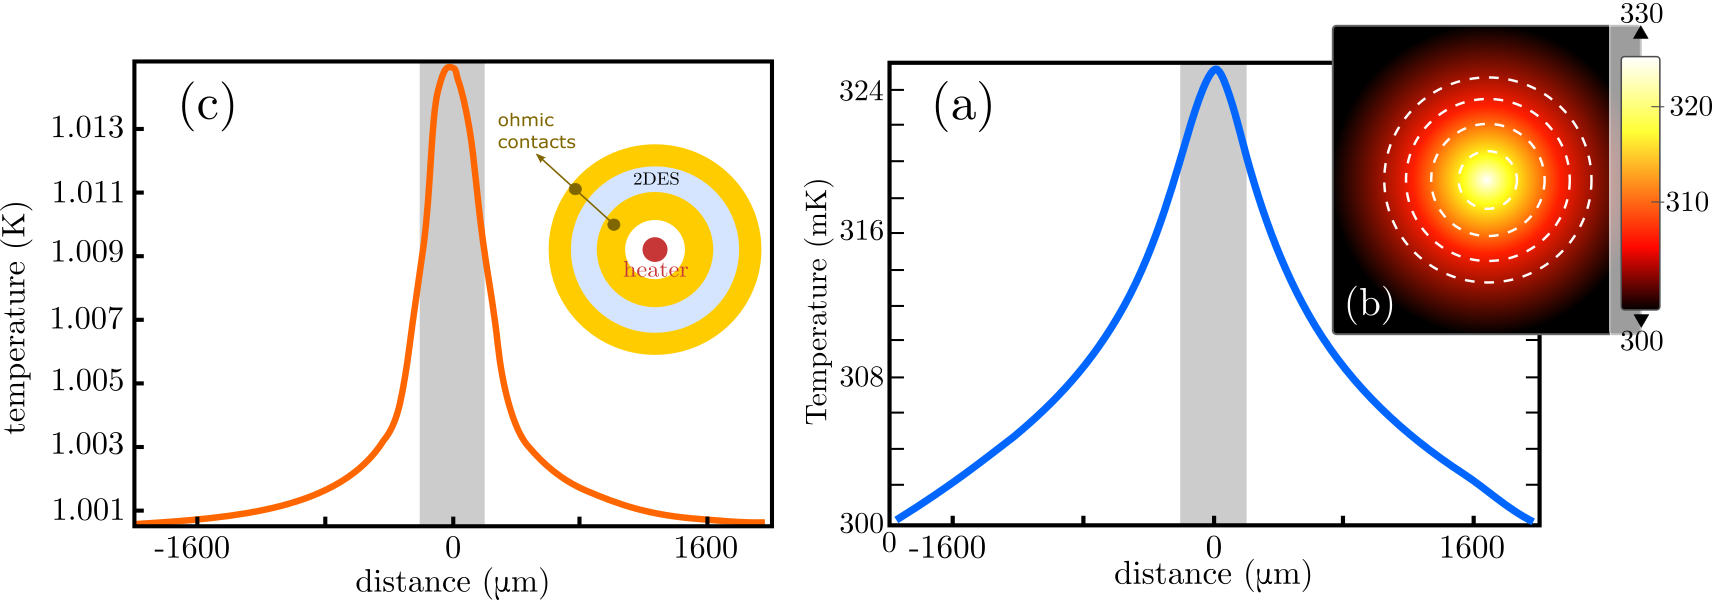
\includegraphics[width=1\textwidth]{figures/experimental/comsol_helium_dry_and_wet.png}
    \caption{Simulation of both (c) wet and (a) dry systems, it is assumed that a a point heater induces a power on a GaAs crystal. The borders of the sample are anchored in both cases. But in the case of the wet system the Helium thermal conductivity is also included. Possible radiation is discussed in the text. Gray area indicates the etched central mesa area in the samples. (b) shows a 2D profile of the expected temperature.}
    \label{fig:comsolHelium}
\end{figure}


\textcolor{red}{tenemos algunas mediciones de INTI que sería interesante incluir, pero va a volverse todo largo y no las utilizamos en las publicaciones. Lo que aprendimos acá nos ayudó a llevar a cabo las medicones allá y configurar los equipos de forma correcta. No sé cuánto incluir de esto y si tiene sentido o no. Personalmente creo que es bueno indicar al menos las cosas que no funcionan para que otro se salve de probarlas, o incluso las pueda llevar acabo con mejoras.}

As we have said the thermovoltage measurements are well defined when we use an ideal (infinite) input impedance. In the case of the LL, when the system is acting basically as a metal, it should be enough to use some standard measurement configuration. But, once we reach quantization, i.e. when measuring in the gap, the impedance becomes a much important deal. In the gap, the system presents an almost null conductance, in the order of \textcolor{red}{meter valor conductance}, to overcome this problem several configurations were tested resulting in the use of the differential DC amplifier sketched in the setup of Fig.~\ref{fig:corbino_exp_setup}, also a picture is given in Fig. \ref{fig:DCamp}. This is a fixed $\times 1000$ differential amplifier developed specifically for very accurate low noise voltage measurements \cite{Maerki2017}. This instrument had two inputs per channel (top  connectors), so a maximum of two signals per thermovoltage run could be measured. Then two $\times 1000$ amplified output channels are provided (OUT 1 and 2). We will not describe it here but is a very interesting device as explained in its describing work \cite{Maerki2017}. 

\begin{figure}
    \centering
    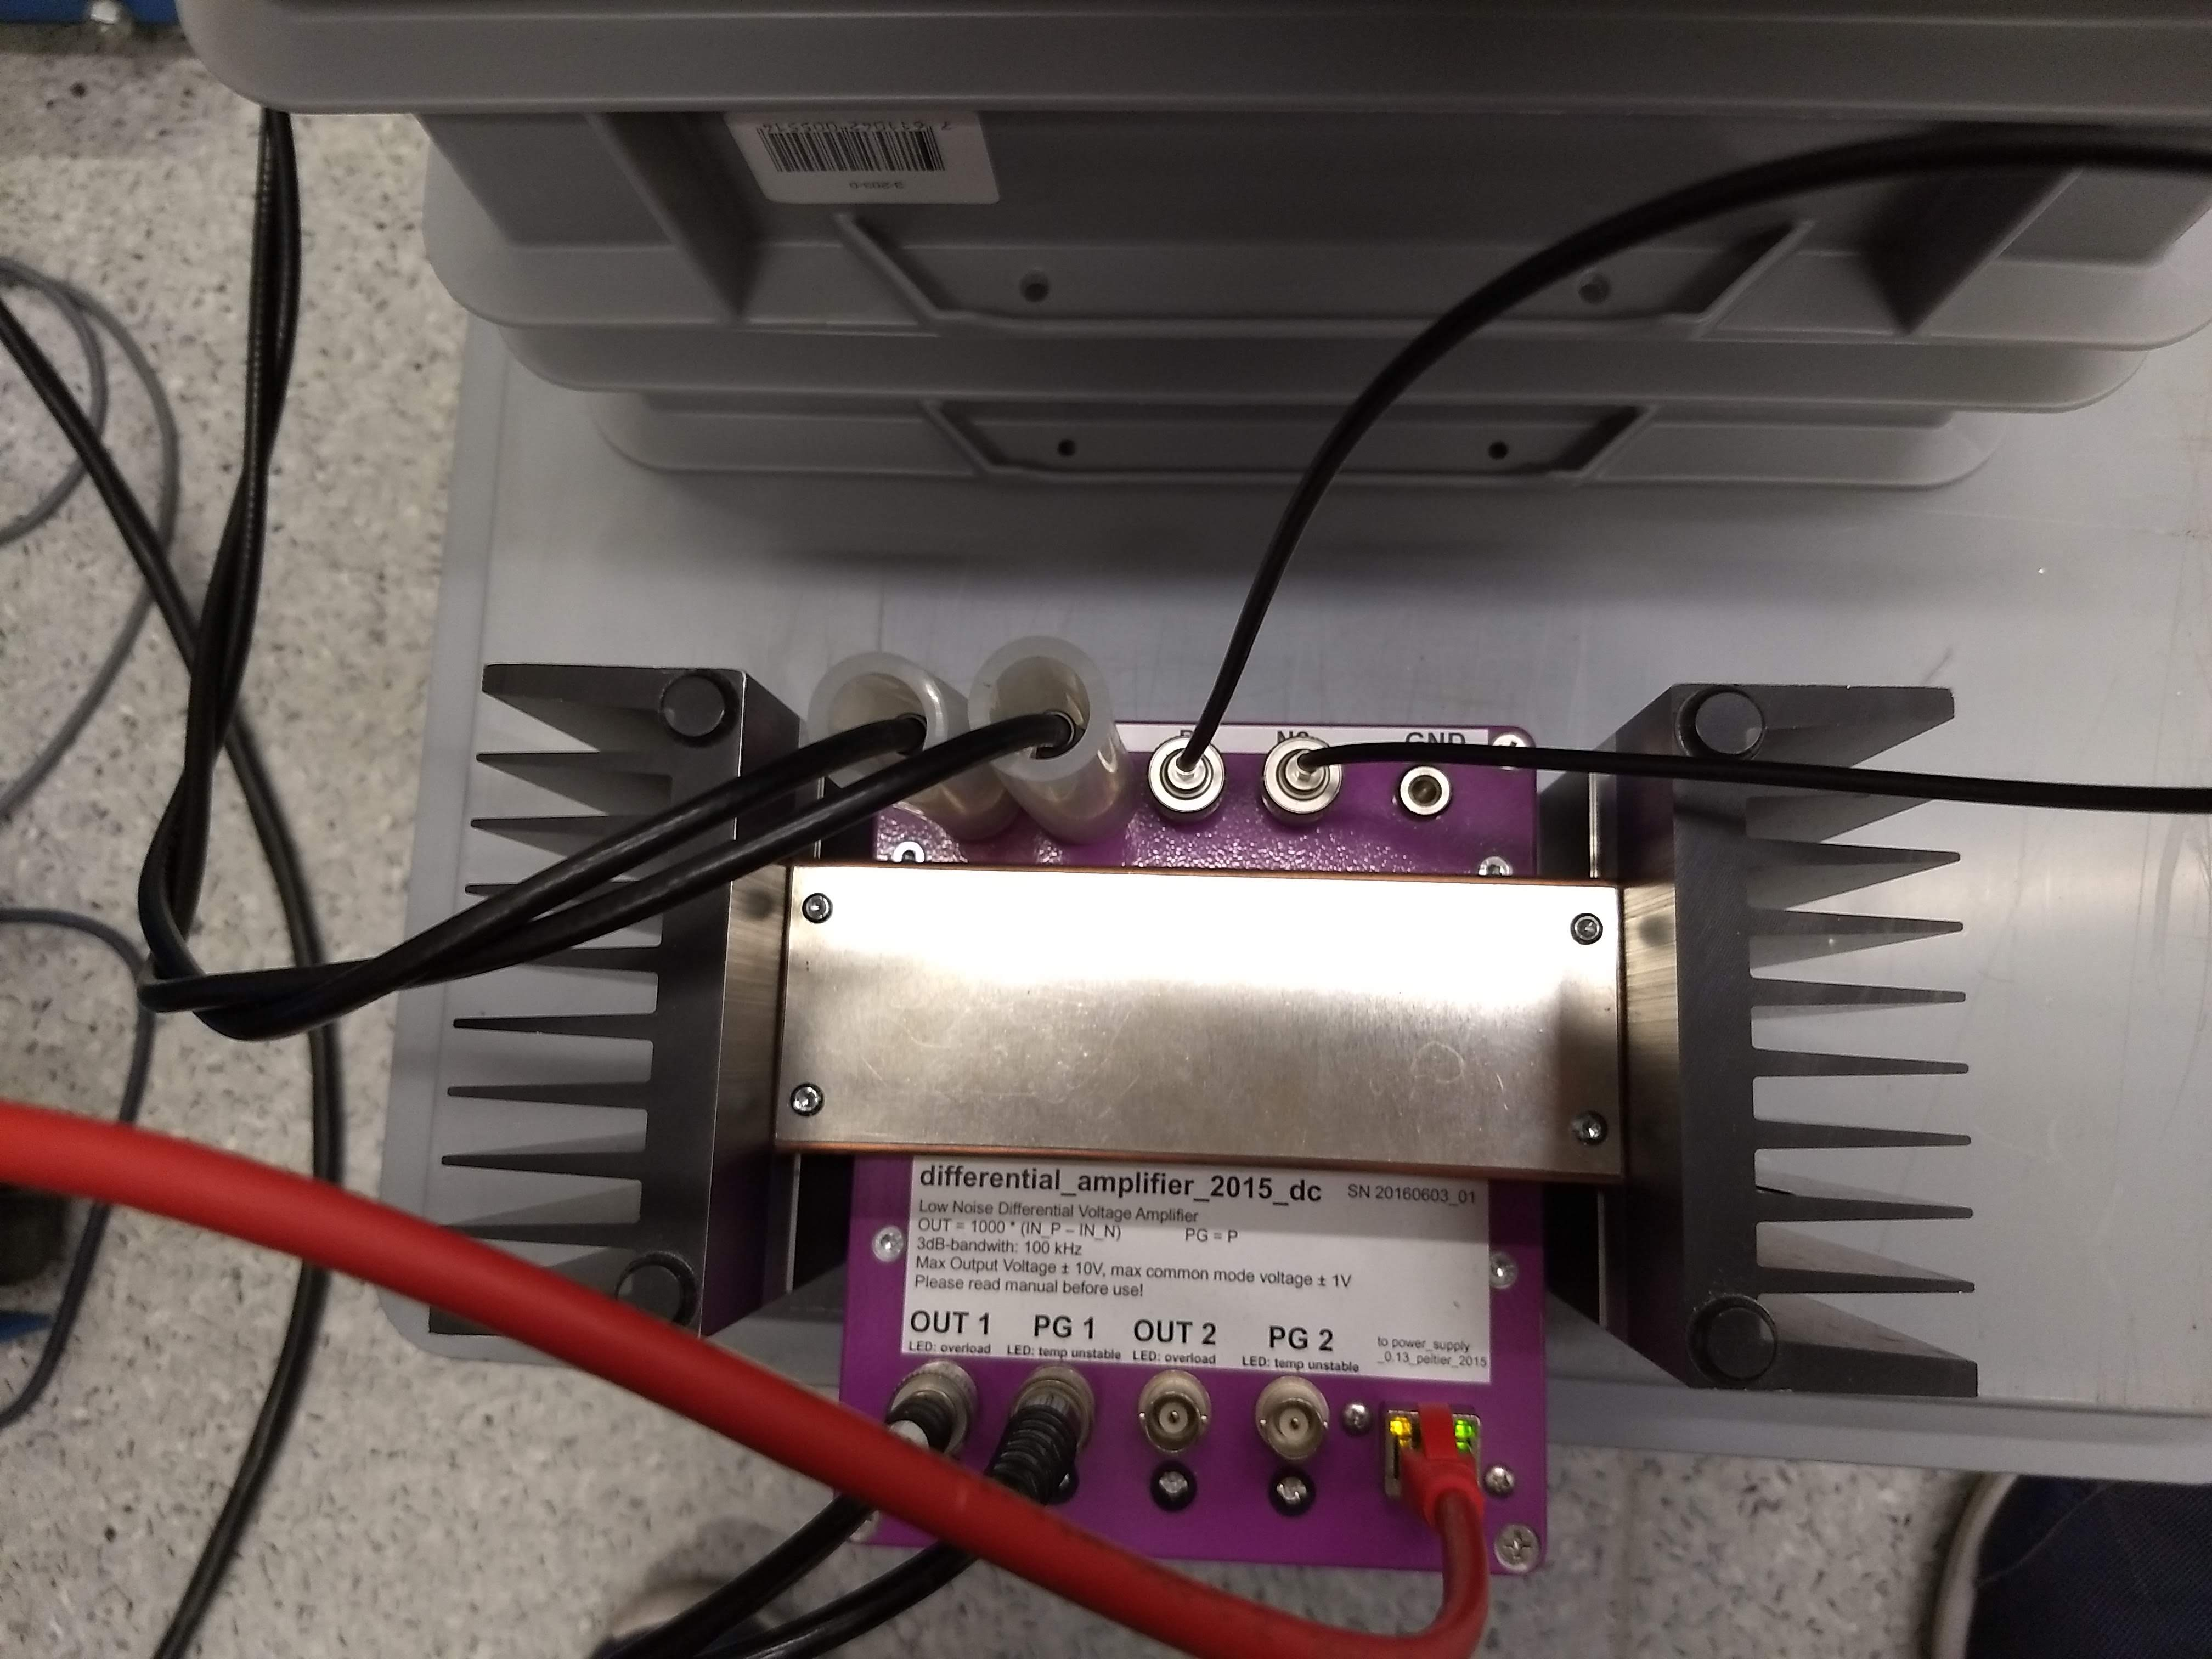
\includegraphics[width=0.6\textwidth]{figures/experimental/DCamp2.jpg}
    \caption{Image of the DC amplifier used for the  \( \vtp \) measurements. The use of BNCs is not the best approach, but it was the standard used in the laboratory. Note the protection in the input (left) terminals, this avoids thermal currents and possible touching to modify the voltage measurements. 
    The PG outputs allows to measure the one of the inputs to the internal amplifier, finally the RJ45 is the power input.  \textcolor{red}{esto último no sé si es necesario incluirlo, es detalle que usé pero no describo más.}}
    \label{fig:DCamp}
\end{figure}

Given the characteristics of this device it is possible to measure up to \SI{1}{\kilo\hertz} without affecting its performance. 

Many measurement runs were performed to the devices using the configurations described in this chapter. We will return to them in \ref{ch:modeling} in a data driven approach, we shall discuss there our model and how it relates to the measured responses of the different devices. 
